\section{Parte A: Circuito Resonante Serie}

\subsection{Objetivos y Fundamento Teórico}
El objetivo de esta sección es estudiar el comportamiento de un circuito $RLC$ serie al modificar la frecuencia de la fuente de alimentación. La ecuación general que gobierna la tensión en este circuito está dada por:
\begin{equation}
V = I \left[ R + j\left(\omega L - \frac{1}{\omega C}\right) \right]
\end{equation}

El módulo de la impedancia total $|Z|$ se define como:
\begin{equation}
|Z| = \sqrt{R^2 + \left(\omega L - \frac{1}{\omega C}\right)^2}
\end{equation}

La condición de resonancia ocurre cuando la corriente se encuentra en fase con la tensión, anulando la parte imaginaria de la impedancia compleja. Esto se logra a la frecuencia de resonancia $f_0$:
\begin{equation}
f_0 = \frac{1}{2\pi\sqrt{L \cdot C}}
\end{equation}

Así, conocidos los valores de frecuencia de resonancia y el valor del capacitor, se puede determinar la inductancia del inductor desconocido:

\begin{equation}
L = \frac{1}{(2\pi f_0)^2 C}
\label{calculo_l_1}
\end{equation}

En este punto, la corriente eficaz alcanza su valor máximo, $I_0 = \frac{V}{R}$, comportándose el circuito de forma puramente resistiva. El factor de calidad o coeficiente de mérito $Q$ determina la agudeza de la curva de resonancia en función del ancho de banda ($BW = f_2 - f_1$):
\begin{equation}
Q = \frac{f_0}{f_2 - f_1} = \frac{\omega_0 L}{R}
\label{calculo_q}
\end{equation}

Podemos ver que sabiendo el factor de calidad y la resistencia utilizada, se puede determinar de otra forma la inductancia del inductor desconocido:
\begin{equation}
L = \frac{Q \cdot R}{\omega_0}
\end{equation}

\subsection{Resultados Experimentales y Análisis}
Se armó un circuito RLC serie con un resistor $R = 773\,\Omega$ y un capacitor $C = 74\,\text{nF}$ conocidos, junto a un inductor L de valor desconocido (Figura \ref{fig:parteA}). Se conectó el circuito a una fuente de tensión alterna de $V_{in}$ = $12\,\text{V}$ pico a pico y se midió la tensión pico a pico ($V_R$) sobre el resistor para distintas frecuencias.

\begin{figure}[H]
\centering
\begin{circuitikz}[american]
    \draw (0,0) to[sinusoidal voltage source, l=$V_{in}$] (0,3) to[R, l=$R$] (3,3) to[L, l=$L$] (3,0) to[C, l=$C$] (0,0);
\end{circuitikz}
\caption{Esquema del circuito RLC serie utilizado en la Parte A.}
\label{fig:parteA}
\end{figure}

Los datos obtenidos se presentan en la Tabla \ref{tab:parteA} y se grafican en la Figura \ref{fig:comparacion_RLC}, donde se observa claramente un pico de tensión en $f_0 = 2.7\,\text{kHz}$, confirmando la condición de resonancia.

\begin{table}[H]
\centering
\caption{Valores de tensión sobre la resistencia en función de la frecuencia.}
\label{tab:parteA}
\begin{tabular}{ccc}
\toprule
$N^{\circ}$ & Frecuencia [kHz] & Tensión $V_R$ [Vpp] \\
\midrule
1  & 0.307                & 0.856 \\
2  & 0.533                & 1.46  \\
3  & 1.03              & 2.80  \\
4  & 1.53 (Corte $f_1$)& 4.27  \\
5  & 1.57               & 4.28  \\
6  & 2.1                & 5.64   \\
7  & 2.7  (Resonancia)  & 6.04   \\
8  & 2.95               & 5.96   \\
9  & 3.5                & 5.60   \\
10 & 4.27               & 4.96   \\
11 & 5.00  (Corte $f_2$)& 4.27   \\
12 & 6.28               & 3.52   \\
13 & 12.7               & 1.84   \\
\bottomrule
\end{tabular}
\end{table}

\begin{figure}[H]
\centering
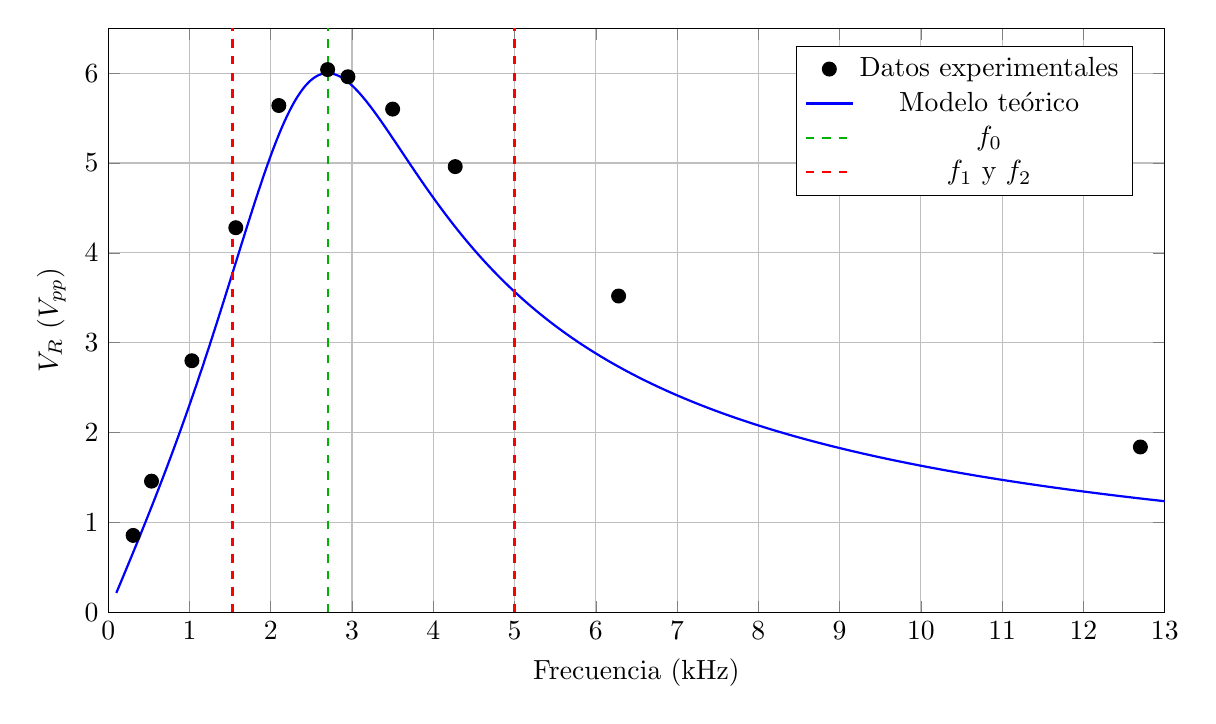
\begin{tikzpicture}
\begin{axis}[
    width=15cm,
    height=9cm,
    xlabel={Frecuencia (kHz)}, % <- Cambiado a kHz
    ylabel={$V_R$ ($V_{pp}$)},
    xmin=0,
    xmax=13, % <- Ajustado el rango máximo
    ymin=0,
    ymax=6.5,
    grid=major,
    legend style={at={(0.97,0.97)}, anchor=north east},
    samples=400,
    domain=0.1:13 % <- Ajustado el dominio de la función
]

% Datos experimentales (valores divididos por 1000)
\addplot[
    only marks,
    mark=*,
    mark size=2.5pt
]
coordinates{
(0.307,0.856)
(0.533,1.46)
(1.030,2.80)
(1.570,4.28)
(2.100,5.64)
(2.700,6.04)
(2.950,5.96)
(3.500,5.60)
(4.270,4.96)
(6.280,3.52)
(12.700,1.84)
};
\addlegendentry{Datos experimentales}

% Curva teórica RLC serie (se añade *1000 a la 'x' interna para mantener la escala)
\addplot[
    thick,
    blue
]
{6*773/sqrt(773^2+(2*pi*(x*1000)*0.04696-1/(2*pi*(x*1000)*74e-9))^2)};
\addlegendentry{Modelo teórico}

% Resonancia (2.7 kHz)
\addplot[
    dashed,
    green!70!black,
    thick
]
coordinates {(2.7,0) (2.7,6.5)};
\addlegendentry{$f_0$}

% Corte inferior f1 (1.53 kHz)
\addplot[
    dashed,
    red,
    thick
]
coordinates {(1.53,0) (1.53,6.5)};

% Corte superior f2 (5.0 kHz)
\addplot[
    dashed,
    red,
    thick
]
coordinates {(5,0) (5,6.5)};
\addlegendentry{$f_1$ y $f_2$}

\end{axis}
\end{tikzpicture}
\caption{Comparación entre la respuesta experimental y la respuesta teórica del circuito RLC serie.}
\label{fig:comparacion_RLC}
\end{figure}

Podemos observar que la curva teórica se ajusta razonablemente bien a los datos experimentales, aunque existen pequeñas discrepancias que pueden atribuirse a las tolerancias de los componentes y a las pérdidas no consideradas en el modelo ideal. La frecuencia de resonancia $f_0$ se identificó claramente, asi como los puntos de corte $f_1$ y $f_2$, con lo que podemos afirmar que el circuito se comporta de acuerdo a las predicciones teóricas para un circuito RLC serie.
\newline

A partir de la curva de respuesta, se identificó experimentalmente la frecuencia de resonancia en $f_0 = 2.7\text{ kHz}$. Asi, utilizando la ecuación \ref{calculo_l_1}, se calculó la inductancia del inductor desconocido:

\begin{equation}
L = \frac{1}{(2\pi f_0)^2 C} = 46.96\text{ mH}
\end{equation}

Luego, utilizando las frecuencias de corte de media potencia para las cuales la tension sobre la resistencia cae a $V_R/\sqrt{2}$ = $4.27\text{ V}$ ($f_1 = 1.53\text{ kHz}$ y $f_2 = 5\text{ kHz}$), se determino el factor de calidad del circuito a partir de la ecuacion \ref{calculo_q} para las frecuencias de corte:
\begin{equation}
Q = \frac{f_0}{f_2 - f_1} = 0.778
\end{equation}

A partir de este valor, se pudo calcular nuevamente la inductancia del inductor desconocido utilizando la ecuación \ref{calculo_q} para el factor de calidad:
\begin{equation}
L = \frac{Q \cdot R}{\omega_0} = 35.45\text{ mH}
\end{equation}

Este segundo valor de inductancia se encuentra en el mismo orden de magnitud que el calculado a partir de la frecuencia de resonancia, aunque con una diferencia significativa. Esta discrepancia puede atribuirse a la presencia de pérdidas adicionales en el circuito, como la resistencia interna del inductor o las pérdidas dieléctricas del capacitor, que no fueron consideradas en el modelo teórico ideal.